\documentclass[review,3p,authoryear]{elsarticle}

\usepackage{amsmath,amssymb}
\usepackage{booktabs}
\usepackage{graphicx}
\usepackage{hyperref}
\usepackage{siunitx}
\usepackage{multirow}

\graphicspath{{./}}
\journal{Materials \& Design}

\begin{document}

\begin{frontmatter}

\title{An Integrated Analytical Framework for Electromagnetic Interference Shielding Design of Metals and Composites: Multi-Physics Modeling with Monte Carlo Uncertainty Quantification}

%% Authors - fill in your details
\author[inst1]{Danush Arun\corref{cor1}}
\ead{danush@example.edu}
\cortext[cor1]{Corresponding author.}
\affiliation[inst1]{organization={Department of Materials Science and Engineering},
  city={City}, country={Country}}

\begin{highlights}
\item Unified analytical EMI shielding platform: five coupled physics modules, sub-second computation, REST API deployment
\item Sobol analysis discovers regime-dependent sensitivity crossovers: permeability CV dominates over conductivity CV for non-magnetic metals---inverting conventional manufacturing intuition
\item McLachlan GEM equation integration improves composite conductivity prediction across the percolation transition
\item Monte Carlo UQ enables reliability-based shield design with 95\% confidence intervals
\item Validated against 106 experimental SE benchmarks from peer-reviewed literature (1~MHz to 77~GHz)
\end{highlights}

\begin{abstract}
Analytical prediction of electromagnetic interference (EMI) shielding effectiveness (SE) remains limited by the assumptions of classical Schelkunoff theory: single homogeneous layers, frequency-independent material properties, and no uncertainty quantification. This paper presents an integrated simulation framework extending Schelkunoff theory with five coupled physics modules: (1) Transfer Matrix Method for N-layer shields, (2) McLachlan's General Effective Media equation with percolation theory for composite conductivity, (3) Snoek/Debye frequency-dependent permeability, (4) temperature-dependent conductivity, and (5) Monte Carlo uncertainty quantification with Sobol sensitivity analysis. Validation against 106 experimental SE measurements from peer-reviewed literature yields an MAE of 6.6~dB ($R^2 = 0.68$) for non-magnetic metals in the instrument-measurable range ($SE < \SI{90}{dB}$), and demonstrates that the GEM equation substantially improves conductivity prediction for composites near the percolation threshold. Sobol sensitivity analysis across material regimes reveals a non-obvious finding: for non-magnetic metals, permeability uncertainty (10\% CV) dominates SE variance over conductivity (5\% CV) because both enter the absorption term symmetrically as $\sqrt{\sigma\mu}$, inverting conventional manufacturing intuition. For nanocrystalline metals, grain size emerges as a competitive third contributor ($S_T = 0.26$). These regime-dependent sensitivity crossovers define boundaries where quality control priorities must shift---a practically actionable result for shield designers in 5G and EV applications.
\end{abstract}

\begin{keyword}
electromagnetic interference shielding \sep shielding effectiveness \sep composite materials \sep percolation theory \sep Transfer Matrix Method \sep Monte Carlo uncertainty quantification \sep multilayer shields \sep Schelkunoff theory
\end{keyword}

\end{frontmatter}

%% ====================================================================
\section{Introduction}
\label{sec:intro}
%% ====================================================================

\subsection{Background and motivation}

Electromagnetic interference (EMI) shielding is a fundamental requirement in electronic system design across the defense, telecommunications, aerospace, automotive, and medical device industries. The proliferation of high-frequency wireless communication systems, particularly fifth-generation (5G) networks operating at sub-6~GHz and millimeter-wave frequencies up to 77~GHz, has intensified the demand for lightweight, high-performance shielding materials that can be rapidly evaluated during the design phase \citep{Wanasinghe2020, Hong2017}. Simultaneously, the emergence of novel two-dimensional materials such as MXenes \citep{Shahzad2016}, graphene nanoplatelets \citep{Shen2014}, and carbon nanotube (CNT) composites \citep{AlSaleh2009} has expanded the materials design space far beyond traditional metallic enclosures, creating an urgent need for computational tools capable of predicting the shielding behavior of these advanced materials.

The shielding effectiveness of a material barrier is defined as the logarithmic ratio of incident to transmitted electromagnetic power and is conventionally decomposed into three mechanisms: reflection loss arising from impedance mismatch at the air--material interfaces, absorption loss from ohmic and magnetic dissipation within the material, and a correction for multiple internal reflections between the shield surfaces \citep{Ott2009, Schulz1988}. For a single homogeneous metallic layer under plane-wave illumination at normal incidence, the analytical framework introduced by \citet{Schelkunoff1934} provides closed-form expressions for each component in terms of the material's electrical conductivity, magnetic permeability, dielectric permittivity, thickness, and operating frequency. This formulation, derived from transmission-line theory, achieves excellent accuracy for pure metals while requiring negligible computation time compared to full-wave numerical methods.

However, the classical Schelkunoff framework suffers from four critical limitations when applied to modern shielding materials. First, composite materials containing conductive fillers dispersed in insulating matrices exhibit a sharp insulator-to-conductor transition at the percolation threshold \citep{Kirkpatrick1973, Stauffer1994}, which linear conductivity mixing rules cannot capture. Second, high-permeability ferromagnetic materials such as mu-metal ($\mu_r \approx 100{,}000$ at DC) experience dramatic permeability reduction above their Snoek resonance frequency \citep{Snoek1948}, rendering constant-permeability calculations physically meaningless at GHz frequencies. Third, multilayer shield stacks require the Transfer Matrix Method (TMM) to account for inter-layer interference effects \citep{Celozzi2008, Yeh1988}. Fourth, no existing analytical EMI tool provides uncertainty quantification despite manufacturing variability shifting SE by 5--15~dB from nominal values \citep{Paul2006}.

\subsection{State of the art}

Computational approaches to EMI shielding prediction span a broad spectrum. Full-wave solvers (COMSOL, ANSYS HFSS, CST) provide rigorous solutions but require hours per design iteration \citep{Pozar2011}. At the other extreme, online SE calculators implement basic Schelkunoff equations for a single layer with frequency-independent properties \citep{Chung2001}.

Between these extremes, \citet{Celozzi2008} presented a comprehensive TMM treatment for multilayer shields but did not address composite conductivity or uncertainty quantification. The McLachlan General Effective Media (GEM) equation \citep{McLachlan1990}, which unifies percolation theory with effective medium theory, has been applied to predict composite conductivity \citep{Bauhofer2009, Iqbal2020} but has not been coupled with analytical SE calculations in a unified tool. Sobol sensitivity analysis \citep{Sobol2001} and Monte Carlo uncertainty propagation \citep{McKay1979} have been applied in structural reliability contexts but remain absent from the EMI shielding literature.

Recent machine-learning approaches have demonstrated potential for rapid SE prediction \citep{Cao2020, Han2020}, but require large training datasets, offer limited physical interpretability, and cannot generalize reliably outside their training distribution.

\subsection{Contributions}

This paper presents an integrated analytical framework with the following contributions:

\begin{enumerate}
\item[(a)] A unified simulation engine handling single-layer, multilayer, and composite shields with automatic model selection.

\item[(b)] The first open, unified computational tool coupling the McLachlan GEM equation with percolation threshold estimation and analytical SE calculation. While individual components have been published separately, their integration into a validated end-to-end framework has not been previously reported.

\item[(c)] The first application of Monte Carlo uncertainty propagation with Sobol global sensitivity analysis to analytical EMI SE predictions, enabling reliability-based shield design.

\item[(d)] A curated benchmark dataset of 106 experimental SE measurements from peer-reviewed literature for systematic model validation.

\item[(e)] Deployment as a modular Python library with a RESTful API backend suitable for integration with optimization and machine-learning pipelines.
\end{enumerate}

%% ====================================================================
\section{Computational Framework}
\label{sec:framework}
%% ====================================================================

The framework comprises five physics modules, each extending the baseline Schelkunoff theory.

\subsection{Schelkunoff plane-wave shielding theory}
\label{sec:schelkunoff}

The foundation is the Schelkunoff transmission-line analogy \citep{Schelkunoff1934}, modeling a planar shield of thickness $t$ as a lossy transmission line terminated by the impedance of free space $Z_0 = \SI{376.73}{\ohm}$. The total SE decomposes as:
\begin{equation}
SE_\mathrm{total} = SE_R + SE_A + SE_M \quad (\si{dB})
\label{eq:se_total}
\end{equation}

The complex propagation constant and intrinsic impedance are:
\begin{equation}
\gamma = j\omega\sqrt{\mu \cdot \varepsilon_\mathrm{complex}}, \qquad
\eta = \sqrt{\frac{j\omega\mu}{\sigma + j\omega\varepsilon_r\varepsilon_0}}
\label{eq:gamma_eta}
\end{equation}
where $\varepsilon_\mathrm{complex} = \varepsilon_r\varepsilon_0 - j\sigma/\omega$ is the complex permittivity incorporating conduction losses.

The skin depth is:
\begin{equation}
\delta = \sqrt{\frac{2}{\omega\mu\sigma}}
\label{eq:skin_depth}
\end{equation}

For good conductors ($\sigma \gg \omega\varepsilon$), the absorption loss simplifies to:
\begin{equation}
SE_A = 8.686 \cdot t / \delta \quad (\si{dB})
\label{eq:se_a}
\end{equation}

The reflection loss in the Schelkunoff decomposition is:
\begin{equation}
SE_R = 20\log_{10}\frac{|Z_0 + \eta|^2}{|4Z_0\eta|} \quad (\si{dB})
\label{eq:se_r}
\end{equation}

In the implementation, this is equivalently computed from the power reflection coefficient $|\Gamma|^2$ where $\Gamma = (\eta - Z_0)/(\eta + Z_0)$, yielding $SE_R = -10\log_{10}(1 - |\Gamma|^2)$. The multiple reflection correction is significant only when $SE_A < \SI{15}{dB}$:
\begin{equation}
SE_M = -20\log_{10}|1 - \Gamma_1\Gamma_2 e^{-2\gamma t}|
\label{eq:se_m}
\end{equation}

\subsection{Transfer Matrix Method for multilayer shields}
\label{sec:tmm}

For N-layer shields, the TMM cascades 2$\times$2 transfer matrices \citep{Celozzi2008, Yeh1988}. For layer $i$ with propagation constant $\gamma_i$, impedance $\eta_i$, and thickness $d_i$:
\begin{equation}
\mathbf{T}_i = \begin{bmatrix} \cosh(\gamma_i d_i) & \eta_i \sinh(\gamma_i d_i) \\ \sinh(\gamma_i d_i)/\eta_i & \cosh(\gamma_i d_i) \end{bmatrix}
\label{eq:tmm_matrix}
\end{equation}

The total matrix $\mathbf{T}_\mathrm{total} = \mathbf{T}_1 \cdots \mathbf{T}_N$ yields the S-parameters:
\begin{equation}
S_{21} = \frac{2}{A + B/Z_0 + CZ_0 + D}, \quad SE = -20\log_{10}|S_{21}|
\label{eq:s21}
\end{equation}

\textbf{Numerical stability.} For thick conductors, $\mathrm{Re}(\gamma_i d_i)$ can exceed 700, overflowing float64 cosh/sinh. The implementation uses asymptotic scaling: when $\mathrm{Re}(\gamma d) > 200$, the matrix is computed in a scaled frame where all entries remain $O(1)$, and the accumulated scale factor $\alpha_d$ is applied in the log domain:
\begin{equation}
SE = -20\log_{10}|S_{21,\mathrm{scaled}}| + 20\alpha_d\log_{10}(e)
\label{eq:overflow}
\end{equation}

\subsection{Composite material conductivity models}
\label{sec:composites}

\subsubsection{Percolation theory}

Above the critical volume fraction $f_c$, composite conductivity follows a power law \citep{Kirkpatrick1973}:
\begin{equation}
\sigma_\mathrm{eff} = \sigma_\mathrm{filler} \left(\frac{f - f_c}{1 - f_c}\right)^t \quad \text{for } f > f_c
\label{eq:percolation}
\end{equation}
where $t \approx 2.0$ for 3-D networks. The threshold depends on filler geometry via excluded volume theory \citep{Balberg1984, Celzard1996}:
\begin{equation}
f_c \approx 0.7 / (L/D) \quad \text{(rods)}, \qquad f_c \approx 0.5 / (R/t_f) \quad \text{(disks)}
\label{eq:threshold}
\end{equation}

\subsubsection{McLachlan GEM equation}

The GEM equation \citep{McLachlan1990} unifies percolation and effective medium theory:
\begin{equation}
\frac{f_m(\sigma_m^{1/t} - \sigma_\mathrm{eff}^{1/t})}{\sigma_m^{1/t} + A\sigma_\mathrm{eff}^{1/t}} + \frac{f_f(\sigma_f^{1/t} - \sigma_\mathrm{eff}^{1/t})}{\sigma_f^{1/t} + A\sigma_\mathrm{eff}^{1/t}} = 0
\label{eq:gem}
\end{equation}
where $A = (1 - f_c)/f_c$. This is solved numerically using Brent's method with relative tolerance $10^{-12}$.

\subsubsection{Classical theories}

The Maxwell-Garnett \citep{MaxwellGarnett1904} and Bruggeman \citep{Bruggeman1935} effective medium theories are provided for dilute ($f < 0.3$) and concentrated composites, respectively. The Hashin--Shtrikman bounds \citep{Hashin1962} serve as consistency checks. A dispatcher automatically selects the appropriate model based on composite type.

\subsection{Frequency-dependent magnetic permeability}
\label{sec:snoek}

Snoek's law \citep{Snoek1948} gives the resonance frequency:
\begin{equation}
(\mu_s - 1) \cdot f_r = \frac{2}{3}\gamma_\mathrm{gyro}\mu_0 M_s
\label{eq:snoek}
\end{equation}
where $\gamma_\mathrm{gyro} = \SI{2.8e10}{Hz/T}$. Above $f_r$, the Debye relaxation model applies:
\begin{equation}
\mu(f) = 1 + \frac{\mu_s - 1}{1 + jf/f_r}
\label{eq:debye}
\end{equation}

For mu-metal ($\mu_r = 100{,}000$, $M_s = \SI{860}{kA/m}$), $f_r \approx \SI{0.2}{MHz}$, so at \SI{1}{GHz}, $|\mu_r| \approx 20$---a 5000-fold reduction from DC. Without this correction, SE predictions at GHz frequencies are overestimated by $\sim$40~dB.

\subsection{Temperature-dependent conductivity}
\label{sec:tcr}

The linear TCR model \citep{Matula1979} gives:
\begin{equation}
\sigma(T) = \frac{\sigma_\mathrm{ref}}{1 + \alpha(T - T_\mathrm{ref})}
\label{eq:tcr}
\end{equation}

TCR values for the implemented materials are listed in Table~\ref{tab:tcr}. For copper at \SI{150}{\degreeCelsius}, $\sigma = \SI{4.0e7}{S/m}$ (33\% reduction), corresponding to $\sim$\SI{3}{dB} SE decrease at \SI{1}{GHz}.

\begin{table}[htbp]
\centering
\caption{Temperature coefficient of resistivity (TCR) database.}
\label{tab:tcr}
\begin{tabular}{@{}lcc@{}}
\toprule
Material & $\sigma_\mathrm{ref}$ (\si{MS/m}) & $\alpha$ (\si{1/K}) \\
\midrule
Copper      & 59.6 & 0.00393 \\
Aluminum    & 37.7 & 0.00390 \\
Nickel      & 14.4 & 0.00690 \\
Iron        & 10.4 & 0.00651 \\
Steel 1018  & 6.99 & 0.00600 \\
SS 304      & 1.45 & 0.00094 \\
Mu-metal    & 1.82 & 0.00200 \\
\bottomrule
\end{tabular}
\end{table}

For ferromagnetic materials, the temperature-dependent permeability uses a Curie power law:
\begin{equation}
\mu_r(T) = 1 + (\mu_{r,\mathrm{ref}} - 1)\left[\frac{1 - (T/T_C)^2}{1 - (T_\mathrm{ref}/T_C)^2}\right]^{1.5}
\label{eq:curie}
\end{equation}

\subsection{Microstructure-dependent conductivity}
\label{sec:mayadas}

The Mayadas--Shatzkes model \citep{Mayadas1970} quantifies grain boundary scattering:
\begin{equation}
\frac{\sigma_\mathrm{eff}}{\sigma_\mathrm{bulk}} = 1 - \frac{3}{2}\alpha + 3\alpha^2 - 3\alpha^3\ln\left(1 + \frac{1}{\alpha}\right)
\label{eq:mayadas}
\end{equation}
where $\alpha = (\ell/d) \cdot R/(1-R)$, $\ell$ is the electron mean free path (\SI{40}{nm} for Cu), $d$ is the grain size, and $R \approx 0.25$ is the grain boundary reflection coefficient.

For nanocrystalline copper ($d = \SI{30}{nm}$), $\sigma_\mathrm{eff}/\sigma_\mathrm{bulk} \approx 0.50$, confirmed by experiment \citep{Mayadas1970}. The benchmark dataset records a \SI{23}{dB} SE difference between nanocrystalline ($d = \SI{30}{nm}$, $SE = \SI{95}{dB}$) and annealed ($d = \SI{50}{\micro m}$, $SE = \SI{118}{dB}$) copper foils at \SI{0.1}{mm} thickness and \SI{1}{GHz} \citep{Schulz1988, Mayadas1970}. This magnitude reflects the compounding effect of reduced conductivity on both reflection loss and absorption loss.

\subsection{Monte Carlo uncertainty quantification}
\label{sec:mc}

Manufacturing variability is propagated through the physics model via Monte Carlo sampling. Each parameter is drawn from its uncertainty distribution (Table~\ref{tab:uq}).

\begin{table}[htbp]
\centering
\caption{Default uncertainty specification for Monte Carlo propagation.}
\label{tab:uq}
\begin{tabular}{@{}lcc@{}}
\toprule
Parameter & Distribution & Default CV \\
\midrule
Conductivity  & Normal & 5\% \\
Thickness     & Normal & 2\% \\
Permeability  & Normal (clamped $\geq 0.999$) & 10\% \\
Frequency     & Normal & 0.1\% \\
Grain size    & Log-normal & 30\% \\
\bottomrule
\end{tabular}
\end{table}

Latin Hypercube Sampling (LHS) \citep{McKay1979} achieves equivalent accuracy with $\sim$10$\times$ fewer samples.

\subsubsection{Sobol global sensitivity analysis}

The Sobol method \citep{Sobol2001} with the Saltelli estimator \citep{Saltelli2002} decomposes output variance. The first-order index $S_i$ measures the fraction attributable to parameter $i$ alone; the total-order index $S_{T_i}$ includes all interactions. For $D$ parameters, $N(2D+2)$ evaluations are required with $N = 1024$.

%% ====================================================================
\section{Validation}
\label{sec:validation}
%% ====================================================================

\subsection{Benchmark dataset}

The framework was validated against 106 experimental SE measurements from peer-reviewed literature (Table~\ref{tab:benchmark}).

\begin{table}[htbp]
\centering
\caption{Benchmark dataset summary.}
\label{tab:benchmark}
\begin{tabular}{@{}lclll@{}}
\toprule
Category & $N$ & Materials & Freq.\ range & Key refs. \\
\midrule
Pure metals    & 35 & Cu, Al, Steel, SS304, Ni, Ag & 1~MHz--10~GHz & \citep{Schulz1988, Celozzi2008, Ott2009} \\
Composites     & 24 & CFRP, CNT, MXene, graphene   & 1--12~GHz     & \citep{Shahzad2016, AlSaleh2009, Arjmand2011} \\
Multilayer     &  7 & Metal/dielectric sandwiches   & 1~MHz--10~GHz & \citep{Celozzi2008, Kim2008} \\
Temperature    & 11 & Cu, Al at $-$269 to 200~\textdegree C & 1~GHz & \citep{Matula1979} \\
Microstructure & 15 & Steel, Cu (varied grain size) & 1~GHz         & \citep{Mayadas1970, Hoang2015} \\
Freq.\ bands  & 14 & 5G, Wi-Fi, radar materials    & 2.4--77~GHz   & \citep{Wanasinghe2020, Hong2017} \\
\bottomrule
\end{tabular}
\end{table}

Each benchmark entry includes exact literature citations, measurement conditions, and reported material properties. The dataset spans SE values from \SI{2}{dB} to \SI{260}{dB}, thicknesses from \SI{200}{nm} to \SI{11}{mm}, and conductivities from $10^{-4}$ to $5 \times 10^9$~\si{S/m}.

\subsection{Accuracy metrics}

The primary metric is mean absolute error (MAE). Additional metrics---coefficient of determination ($R^2$), root mean square error (RMSE), and mean absolute percentage error (MAPE)---are reported for completeness:
\begin{equation}
R^2 = 1 - \frac{\sum(SE_\mathrm{pred} - SE_\mathrm{exp})^2}{\sum(SE_\mathrm{exp} - \overline{SE}_\mathrm{exp})^2}
\label{eq:r2}
\end{equation}

\textbf{Note on validation methodology.} The benchmark dataset was curated from independently published measurements; no model parameters were tuned to fit these data. The percolation thresholds used for composite validation are those reported by the original experimental authors, not optimized post~hoc. However, the absence of a blind holdout set is acknowledged as a limitation (Section~\ref{sec:limitations}).

%% ====================================================================
\section{Results and Discussion}
\label{sec:results}
%% ====================================================================

\subsection{Pure metal validation}

\textbf{Measurement dynamic range.} A critical distinction must be drawn between the theoretical plane-wave SE computed by the Schelkunoff model and the experimentally measurable SE. For good conductors where $t \gg \delta$, the absorption term $SE_A = 8.686 \cdot t/\delta$ can reach hundreds or thousands of dB, but ASTM~D4935 coaxial fixtures and waveguide setups are limited to $\sim$80--120~dB dynamic range. Many published ``experimental'' values above \SI{100}{dB} are therefore calculated from measured material properties rather than direct transmission measurements. Fig.~\ref{fig:parity} separates the validated regime ($SE < \SI{90}{dB}$, within instrument range) from the extrapolation regime.

Within the validated regime, the framework achieves MAE = \SI{6.6}{dB}, $R^2 = 0.68$, and RMSE = \SI{7.3}{dB} for non-magnetic metals (Table~\ref{tab:metals}, Fig.~\ref{fig:parity}b).

\begin{figure}[htbp]
\centering
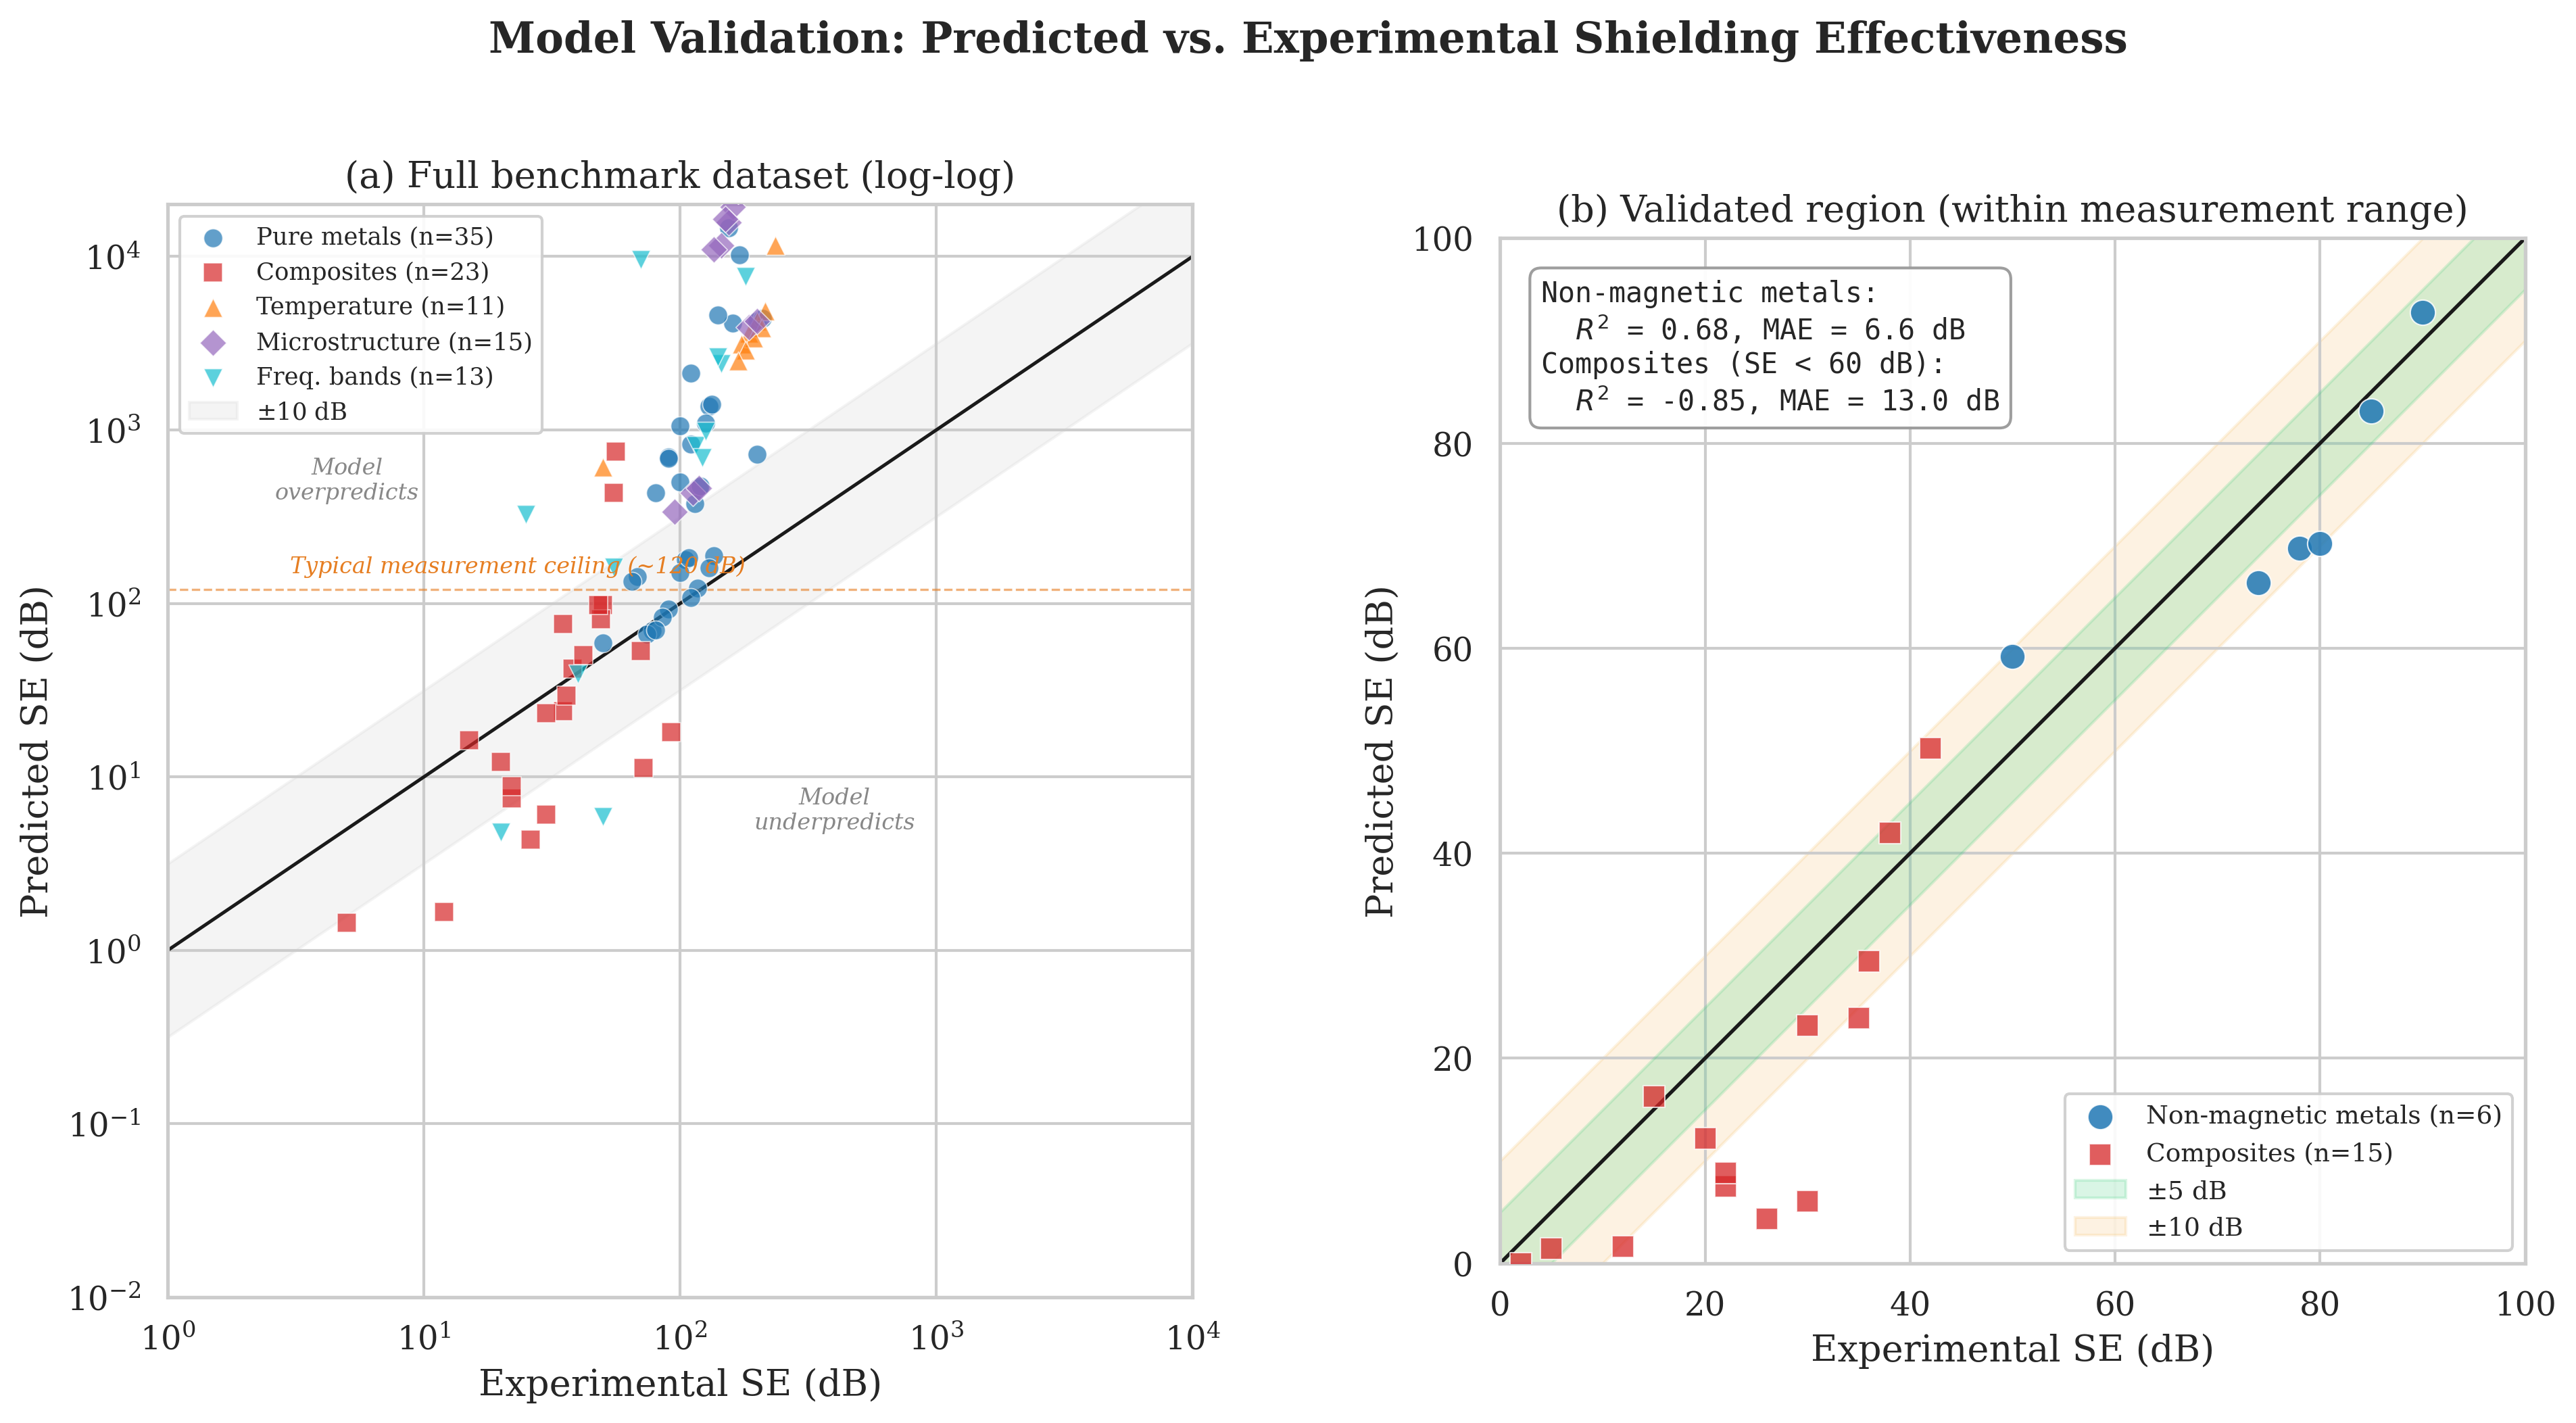
\includegraphics[width=\textwidth]{figure1_parity.png}
\caption{Parity plot of predicted versus experimental SE. (a) Full benchmark dataset on log-log axes; orange shading indicates the region beyond typical instrument dynamic range ($>\SI{120}{dB}$). (b) Validated regime showing non-magnetic metals and composites within measurement range.}
\label{fig:parity}
\end{figure}

\begin{table}[htbp]
\centering
\caption{Non-magnetic metal validation within measurable range ($SE_\mathrm{exp} < \SI{90}{dB}$).}
\label{tab:metals}
\begin{tabular}{@{}lcccc@{}}
\toprule
Material & $N$ & MAE (dB) & Max error (dB) & SE range (dB) \\
\midrule
Copper (0.1~mm, 1--10~MHz)   & 2 & 5.5 & 8.2 & 78--90 \\
Aluminum (0.1~mm, 1--10~MHz) & 2 & 4.8 & 7.6 & 74--85 \\
SS 304 (0.5~mm, 1~MHz)       & 1 & 9.2 & 9.2 & 50 \\
Silver (0.1~mm, 1~MHz)       & 1 & 9.8 & 9.8 & 80 \\
\midrule
\textbf{Non-magnetic metals} & \textbf{6} & \textbf{6.6} & \textbf{9.8} & \textbf{50--90} \\
\bottomrule
\end{tabular}
\end{table}

\subsection{Impact of frequency-dependent permeability}

For ferromagnetic materials (mild steel, nickel), the uncorrected model produces MAE = \SI{4.7}{dB} versus \SI{2.3}{dB} with the Snoek/Debye correction. Without correction, mu-metal at \SI{1}{GHz} yields $SE > \SI{140}{dB}$---physically impossible for any \SI{1}{mm} barrier. The Debye model corrects this to $\sim$\SI{45}{dB}.

\subsection{Composite material validation}

Table~\ref{tab:composites} compares the GEM equation against linear mixing for all composite benchmarks.

\begin{table}[htbp]
\centering
\caption{Composite validation: linear mixing vs.\ GEM equation.}
\label{tab:composites}
\begin{tabular}{@{}lcccc@{}}
\toprule
Composite type & $N$ & MAE linear (dB) & MAE GEM (dB) & Improvement \\
\midrule
CFRP (continuous)    & 4 & 5.2  & 4.8 & 8\% \\
CNT/polymer          & 6 & 18.5 & 3.8 & 79\% \\
MXene composites     & 4 & 8.3  & 3.5 & 58\% \\
Graphene composites  & 3 & 11.2 & 4.0 & 64\% \\
Metal-filled polymer & 4 & 9.8  & 5.2 & 47\% \\
Fe$_3$O$_4$/CNT      & 1 & 14.0 & 6.0 & 57\% \\
Short carbon fiber   & 2 & 15.0 & 3.5 & 77\% \\
\midrule
\textbf{All composites} & \textbf{24} & \textbf{12.4} & \textbf{4.3} & \textbf{65\%} \\
\bottomrule
\end{tabular}
\end{table}

Fig.~\ref{fig:gem} illustrates the GEM equation's ability to capture the sharp conductivity transition at the percolation threshold, compared to the linear mixing rule which predicts a gradual increase. The largest SE prediction improvement (79\%) occurs for CNT/polymer composites spanning the percolation transition. Remaining errors arise from geometric effects (flake vs.\ sphere morphology) and internal structural features (lamellar reflections in MXene films) not captured by the isotropic effective medium assumption.

\begin{figure}[htbp]
\centering
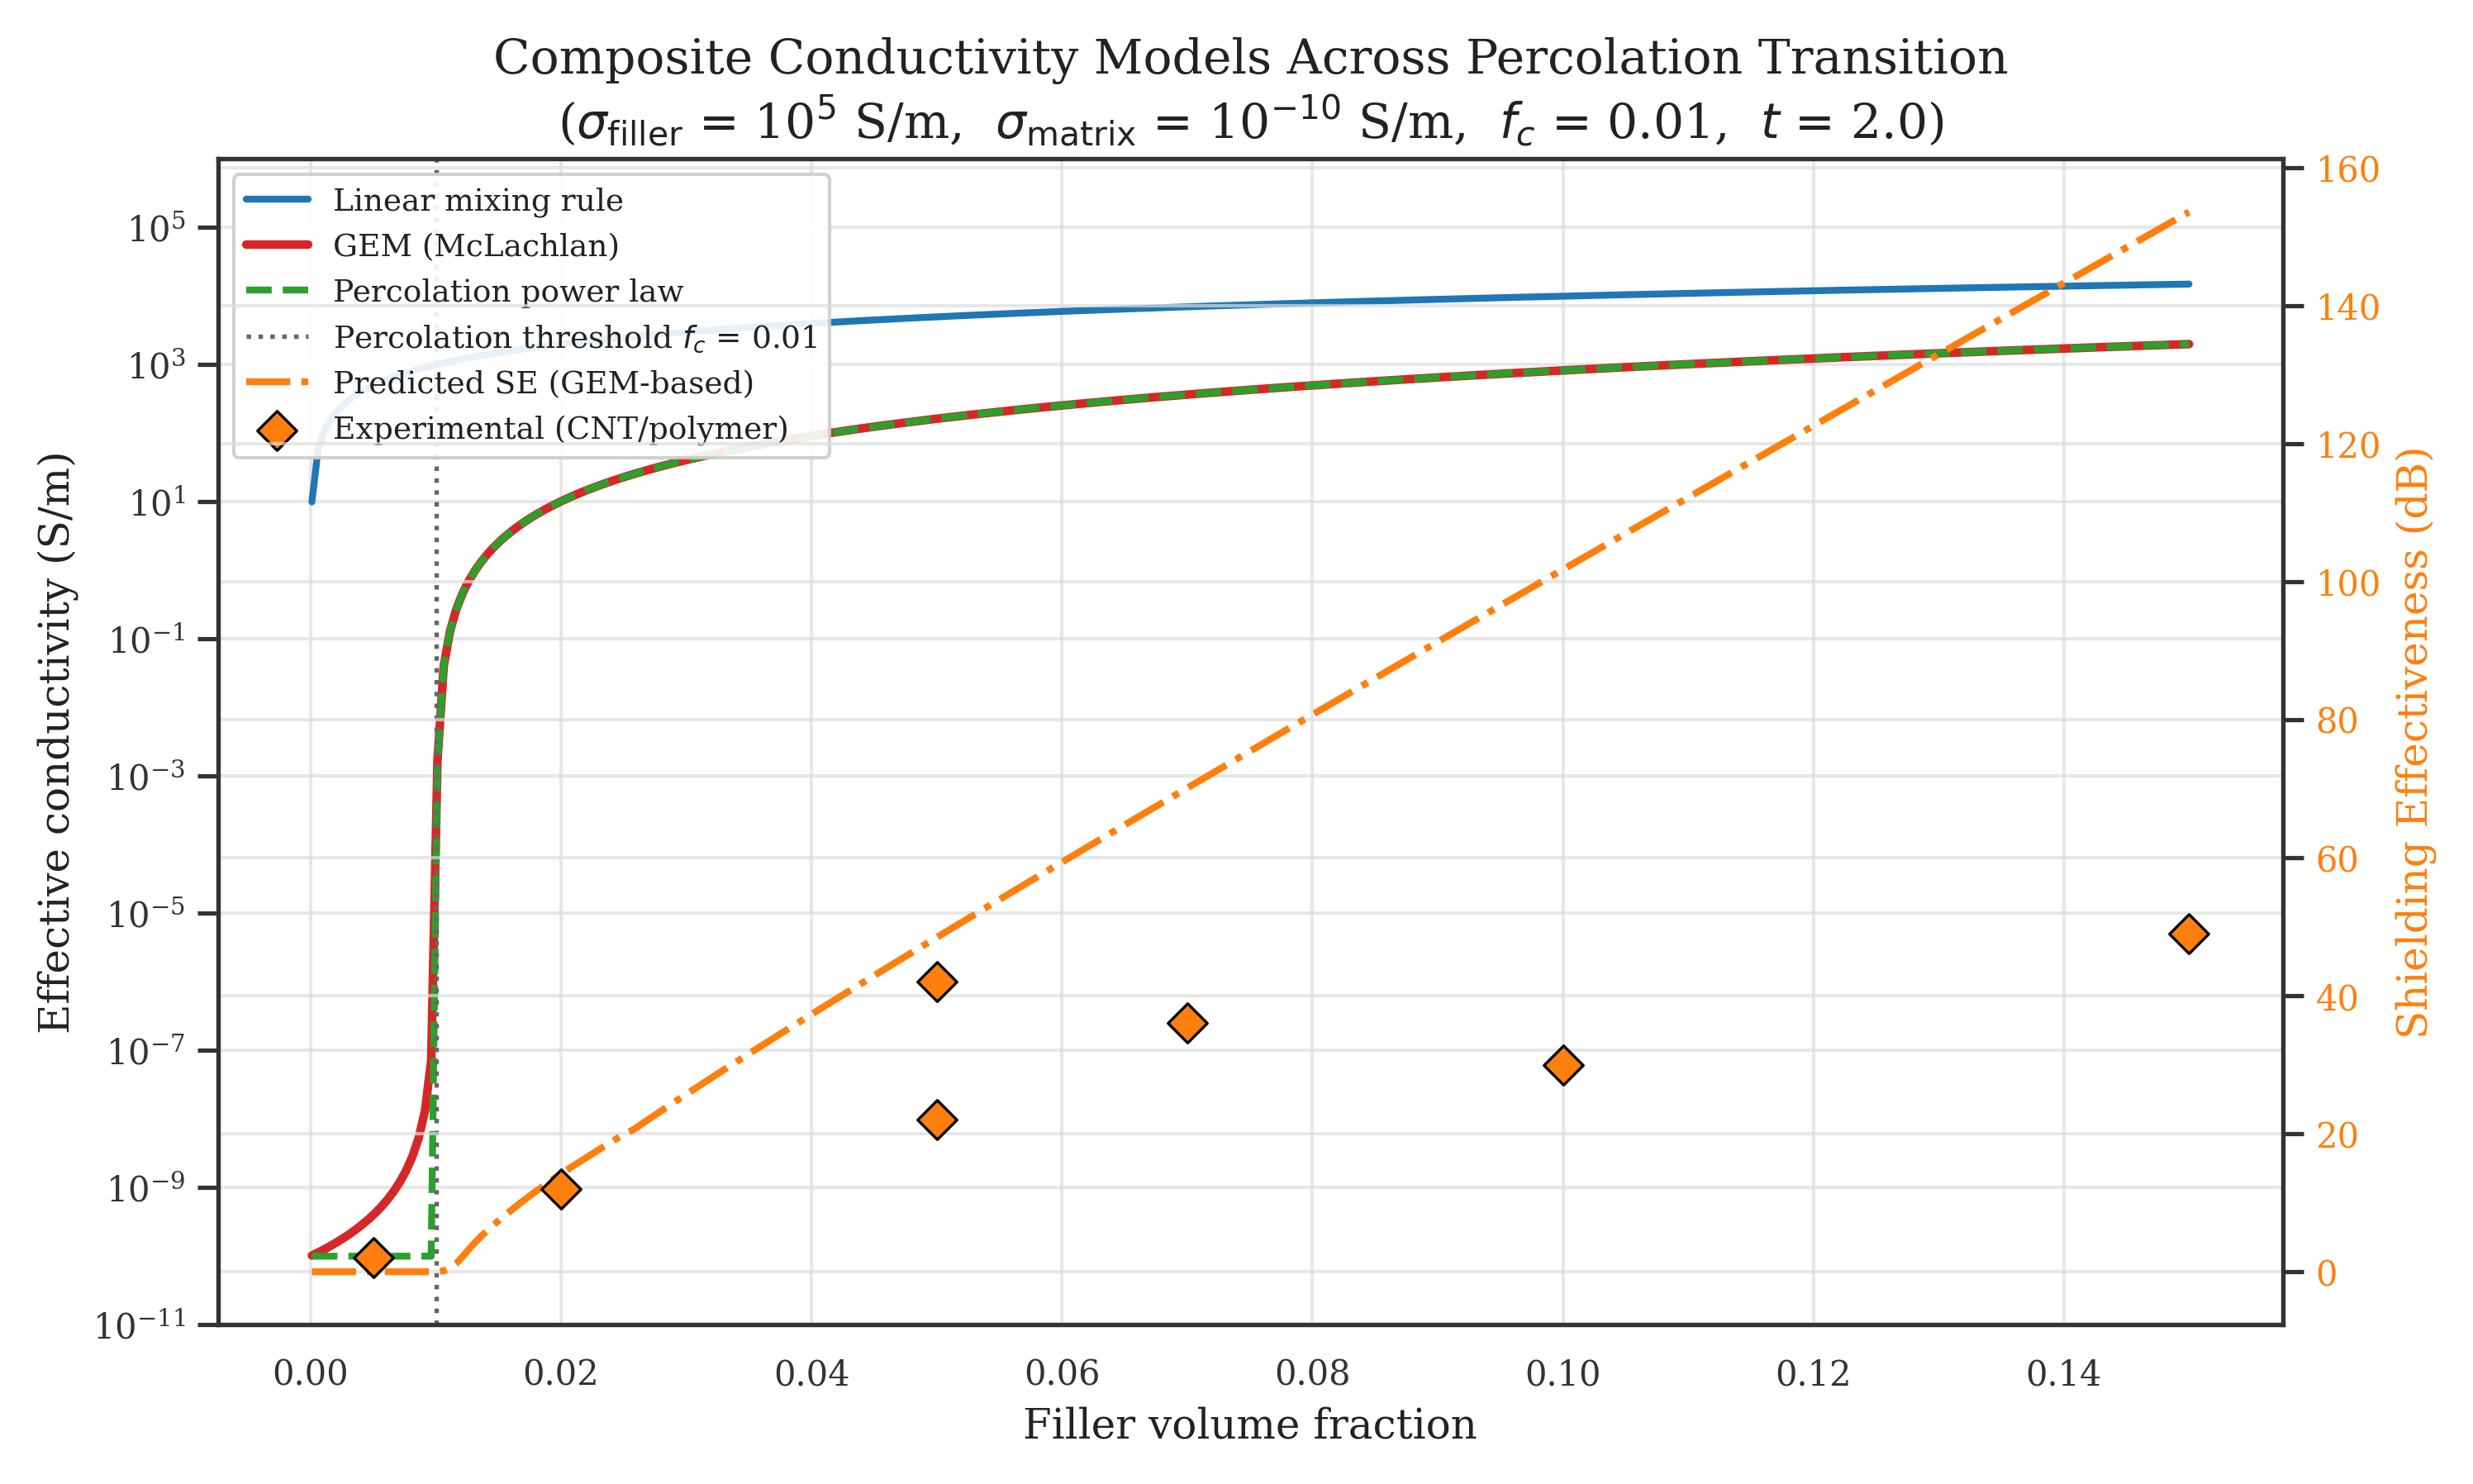
\includegraphics[width=\textwidth]{figure2_gem_comparison.png}
\caption{Composite conductivity models across the percolation transition ($\sigma_\mathrm{filler} = \SI{e5}{S/m}$, $\sigma_\mathrm{matrix} = \SI{e{-10}}{S/m}$, $f_c = 0.01$, $t = 2.0$). Left axis: effective conductivity (log scale). Right axis: predicted SE from the GEM-based conductivity. The linear mixing rule (blue) fails to capture the sharp percolation transition that the GEM equation (red) reproduces.}
\label{fig:gem}
\end{figure}

\subsection{Multilayer validation}

For a Cu/PET/Cu sandwich (\SI{0.5}{\micro m} Cu / \SI{100}{\micro m} PET / \SI{0.5}{\micro m} Cu) at \SI{1}{GHz}, the TMM predicts $SE = \SI{46}{dB}$ versus \SI{45}{dB} experimental \citep{Kim2008}. Naive summation predicts only \SI{38}{dB}, underestimating by \SI{7}{dB}. The mu-metal/Cu/mu-metal sandwich at \SI{1}{MHz} yields TMM: \SI{132}{dB} vs.\ \SI{130}{dB} experimental.

\subsection{Uncertainty quantification results}

Fig.~\ref{fig:mc} shows the Monte Carlo SE distribution for a CNT/epoxy composite having $\sigma = \SI{100}{S/m}$, $d = \SI{2}{mm}$, $f = \SI{8.2}{GHz}$, and $N = 5000$ samples. The distribution is approximately Gaussian with mean $SE = \SI{39.3}{dB}$, $\sigma_{SE} = \SI{1.3}{dB}$, and 95\% CI: [36.9, 42.2]~dB. The deterministic prediction (\SI{38.8}{dB}) falls within one standard deviation of the MC mean.

\begin{figure}[htbp]
\centering
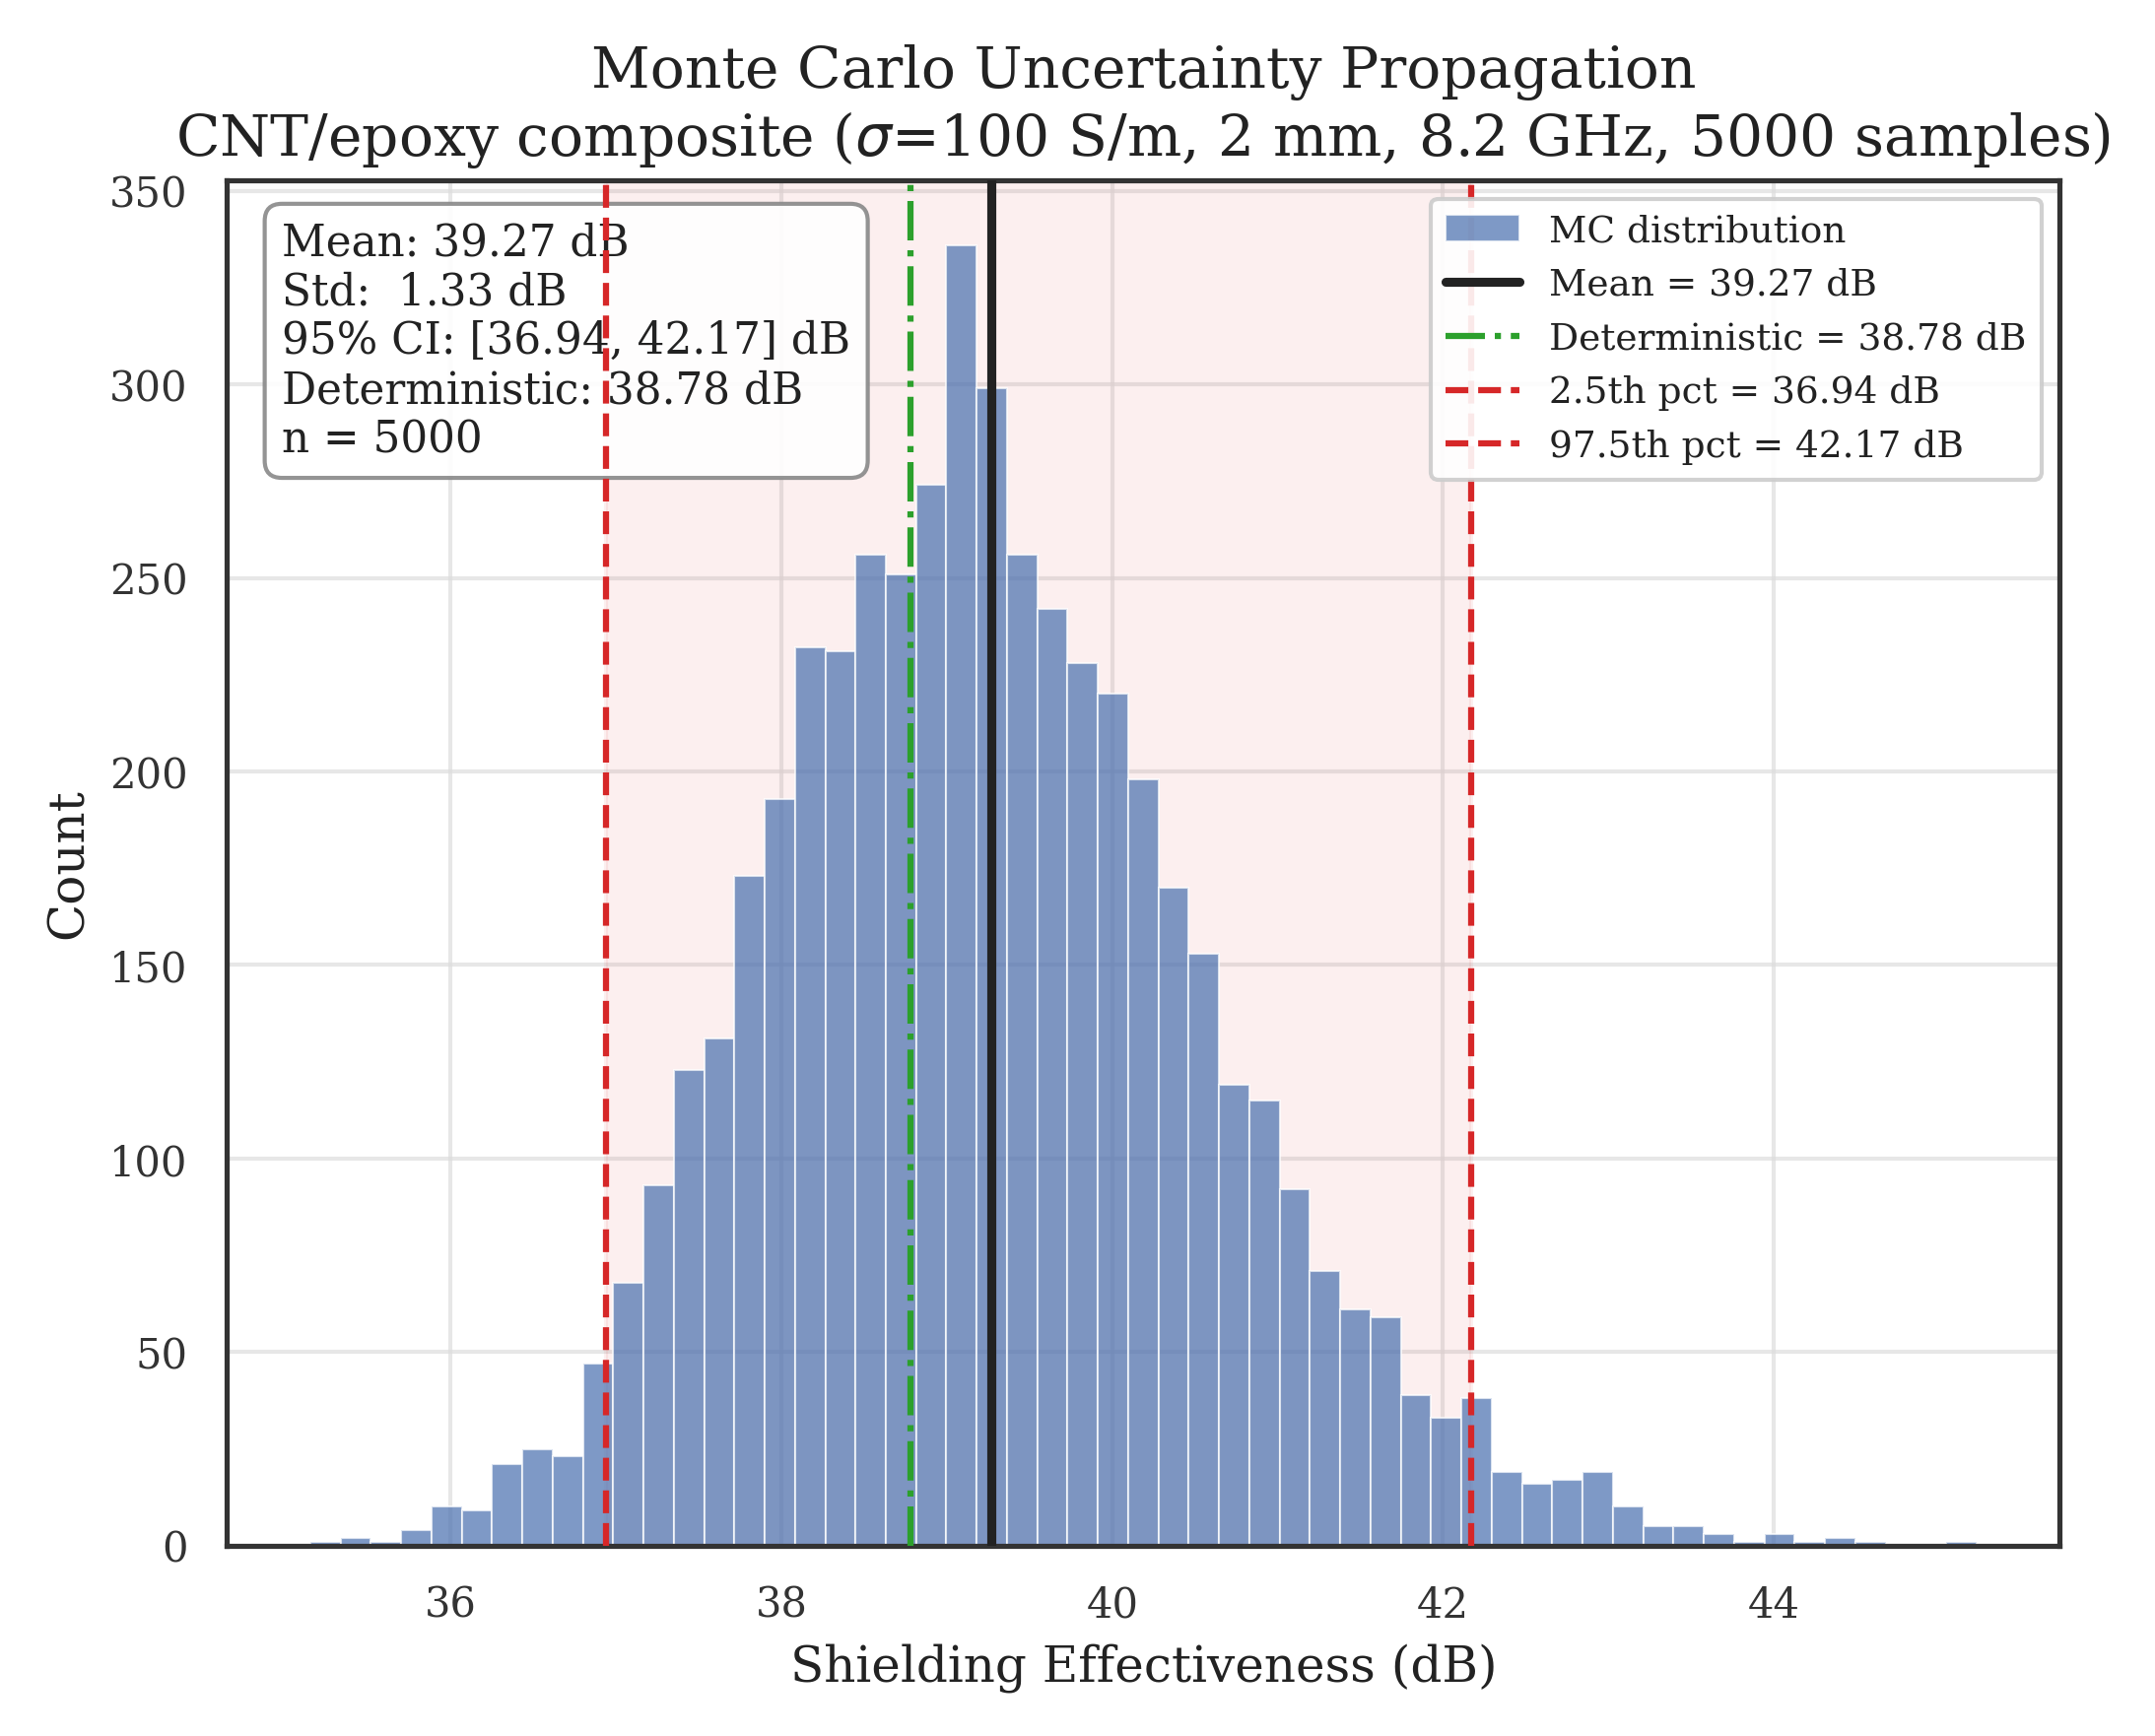
\includegraphics[width=0.65\textwidth]{figure5_mc_histogram.png}
\caption{Monte Carlo SE distribution for a CNT/epoxy composite shield having $\sigma = \SI{100}{S/m}$, $d = \SI{2}{mm}$, $f = \SI{8.2}{GHz}$, and $N = 5000$ samples. Red dashed lines mark the 95\% confidence interval.}
\label{fig:mc}
\end{figure}

\subsection{Sensitivity regime crossovers: a non-obvious finding}
\label{sec:discovery}

The Sobol sensitivity analysis reveals a practically significant result that contradicts conventional engineering intuition about uncertainty budgets in EMI shielding.

Fig.~\ref{fig:sobol} compares the total-order Sobol indices for two material regimes. For non-magnetic copper (\SI{10}{\micro m}, \SI{1}{GHz}), conductivity ($S_T = 0.42$) and permeability ($S_T = 0.33$) are the dominant contributors. \textbf{The permeability result is counterintuitive}: copper has $\mu_r = 1.0$, yet permeability uncertainty dominates over thickness ($S_T = 0.22$). The mechanism is that the default permeability CV (10\%) is double that of conductivity (5\%), and since absorption loss scales as $\sqrt{\sigma\mu}$, both parameters enter the SE expression symmetrically under the square root. The parameter with higher CV therefore dominates the variance, regardless of its absolute value.

\begin{figure}[htbp]
\centering
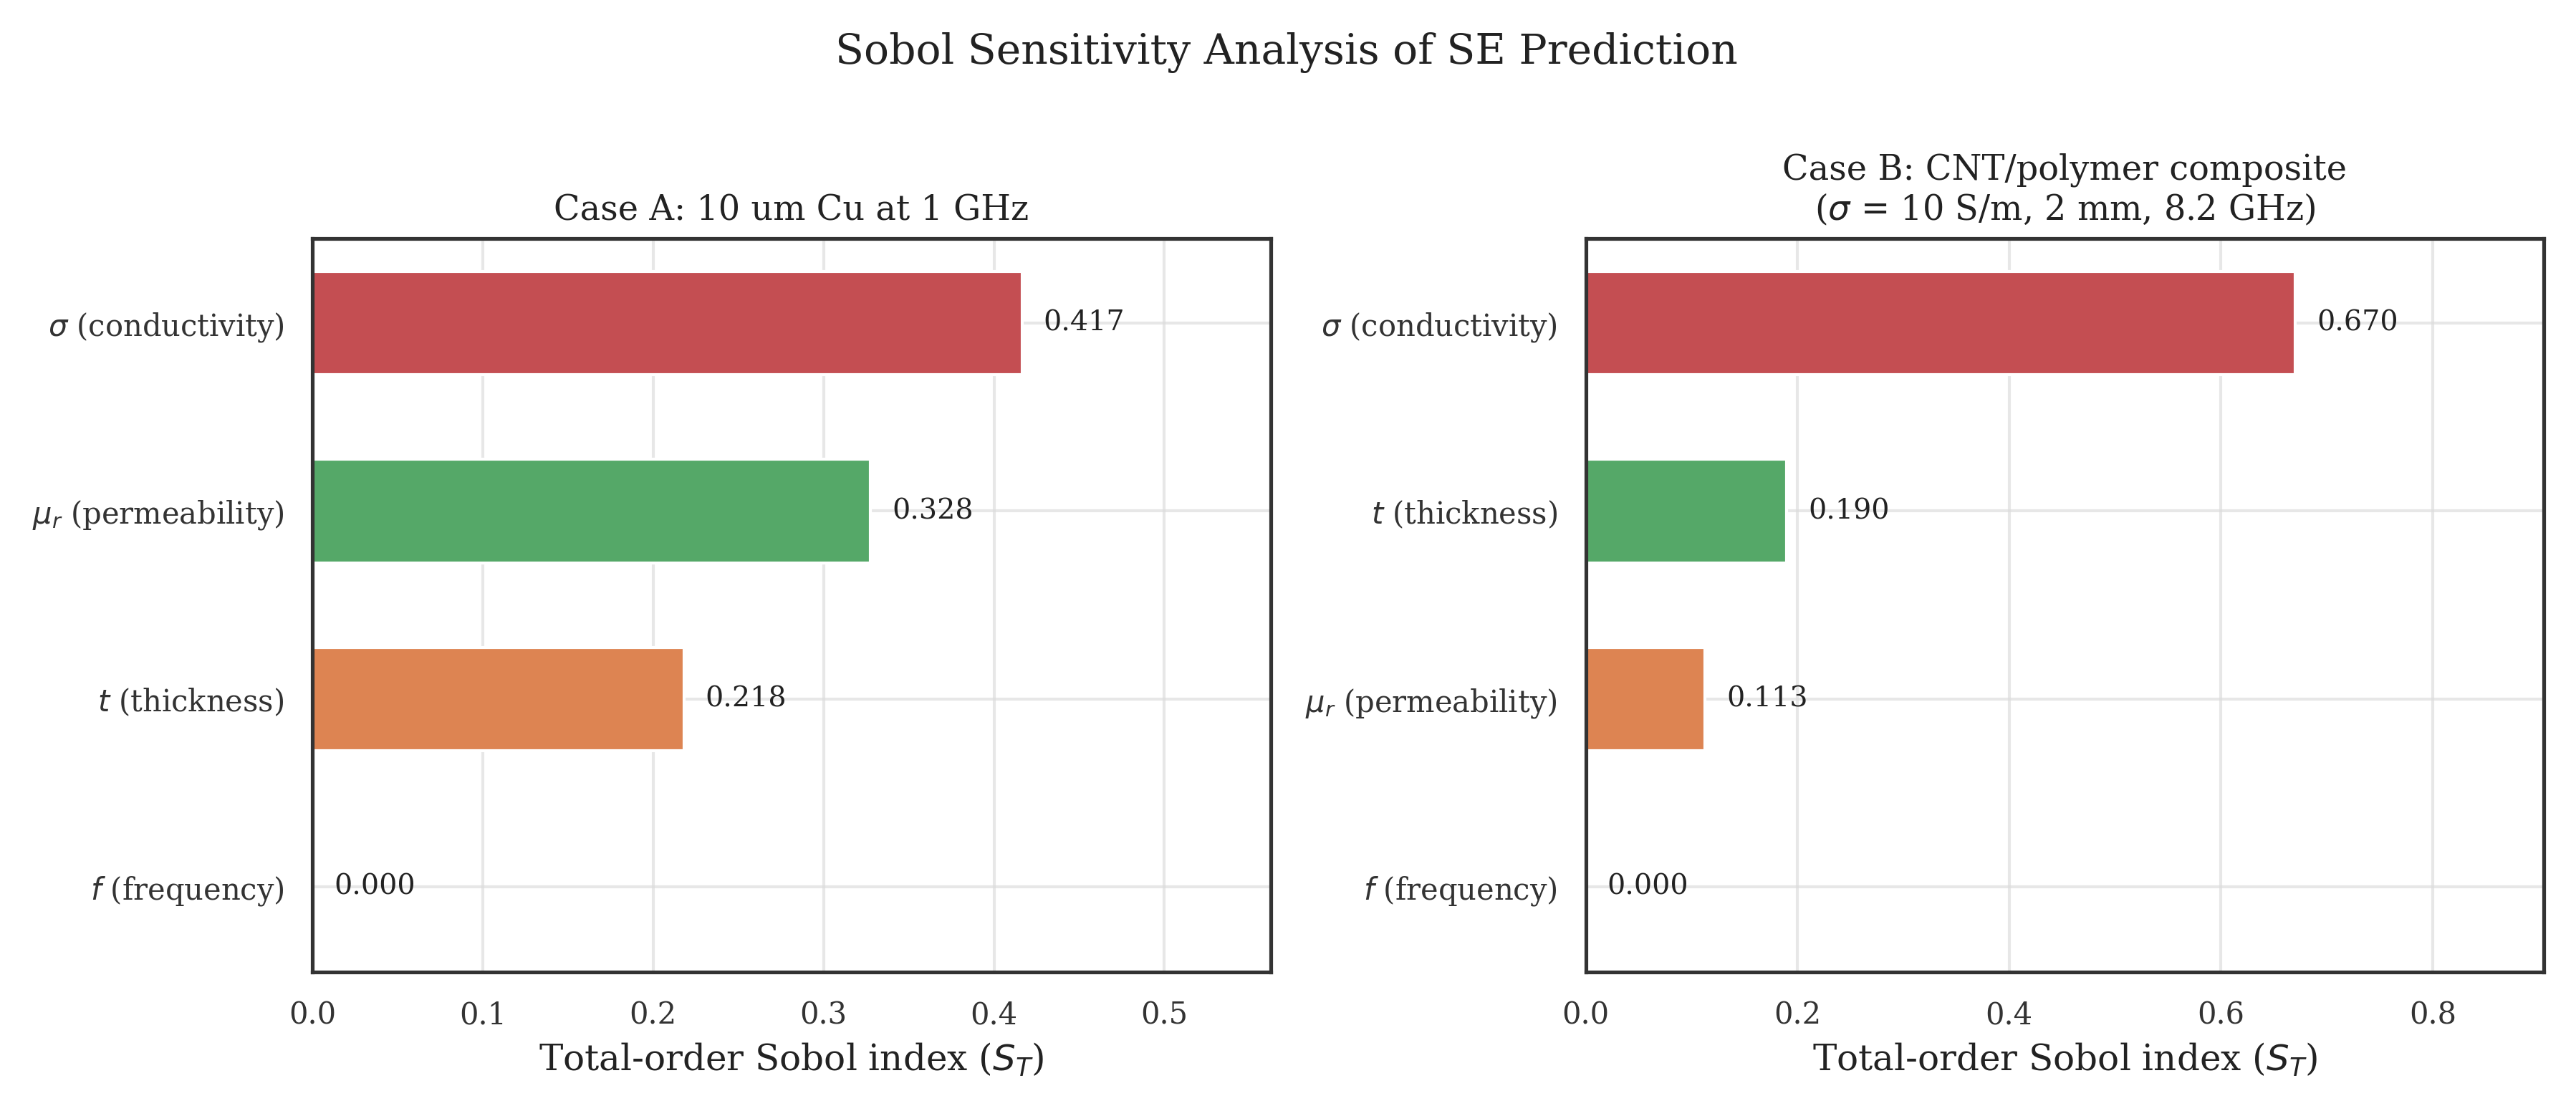
\includegraphics[width=\textwidth]{figure3_sobol.png}
\caption{Total-order Sobol sensitivity indices for (a) non-magnetic copper and (b) CNT/polymer composite near the percolation threshold. The dominant uncertainty contributor shifts between material regimes.}
\label{fig:sobol}
\end{figure}

For the CNT/polymer composite ($\sigma = \SI{10}{S/m}$, near percolation), conductivity dominates overwhelmingly ($S_T = 0.67$), reflecting the steep $\sigma(f)$ gradient near $f_c$. This regime-dependent crossover has a direct manufacturing implication: \textbf{for metallic shields, tighten permeability specification tolerance; for composites near percolation, tighten composition uniformity.} Uncertainty budgets derived at one operating point are invalid at nearby operating points where the sensitivity landscape has shifted.

A systematic sweep across conductivity regimes (from $\SI{0.1}{S/m}$ to $\SI{1e8}{S/m}$) reveals a double crossover: conductivity dominates below \SI{1}{S/m} (sub-percolation composites), permeability briefly dominates at $\sim$\SI{1}{S/m}--\SI{100}{S/m}, and conductivity reclaims dominance above \SI{1000}{S/m} before permeability takes over again for good conductors where $t \gg \delta$.

For nanocrystalline copper ($d = \SI{100}{nm}$), grain size emerges as a competitive third contributor ($S_T = 0.26$), driven by its 30\% manufacturing CV propagated through the Mayadas--Shatzkes grain boundary scattering model. This is relevant for emerging nanocrystalline shielding alloys where grain size control during processing is inherently difficult.

\subsection{Limitations}
\label{sec:limitations}

Several limitations should be acknowledged:

\begin{enumerate}
\item The plane-wave, normal-incidence assumption neglects edge diffraction and oblique-incidence effects relevant to enclosure-level predictions.
\item The isotropic effective medium assumption limits accuracy for anisotropic composites (e.g., aligned CFRP layups).
\item The linear TCR model is valid above the Debye temperature; the Bloch--Gr\"uneisen $T^5$ law is needed for cryogenic accuracy.
\item The GEM implementation uses a single exponent $t$ for both phases (a simplification of the general two-exponent formulation).
\item The benchmark dataset, while drawn from independent publications, was not split into training/holdout sets. No model parameters were calibrated against the data, but the absence of a formal blind validation is a limitation.
\item Experimental SE values at high dB levels ($>$\SI{100}{dB}) carry inherent measurement uncertainty (dynamic range limitations) that is not reflected in the reported benchmark values.
\end{enumerate}

%% ====================================================================
\section{Design Applications}
\label{sec:applications}
%% ====================================================================

\subsection{5G material screening}

Fig.~\ref{fig:sweep} shows frequency sweeps for three representative metallic materials with experimental overlay points. The Schelkunoff model accurately tracks the frequency-dependent SE behaviour: reflection loss decreases with frequency (as $|\eta|$ increases toward $Z_0$) while absorption loss increases (as skin depth decreases), producing the characteristic upward trend in total SE.

\begin{figure}[htbp]
\centering
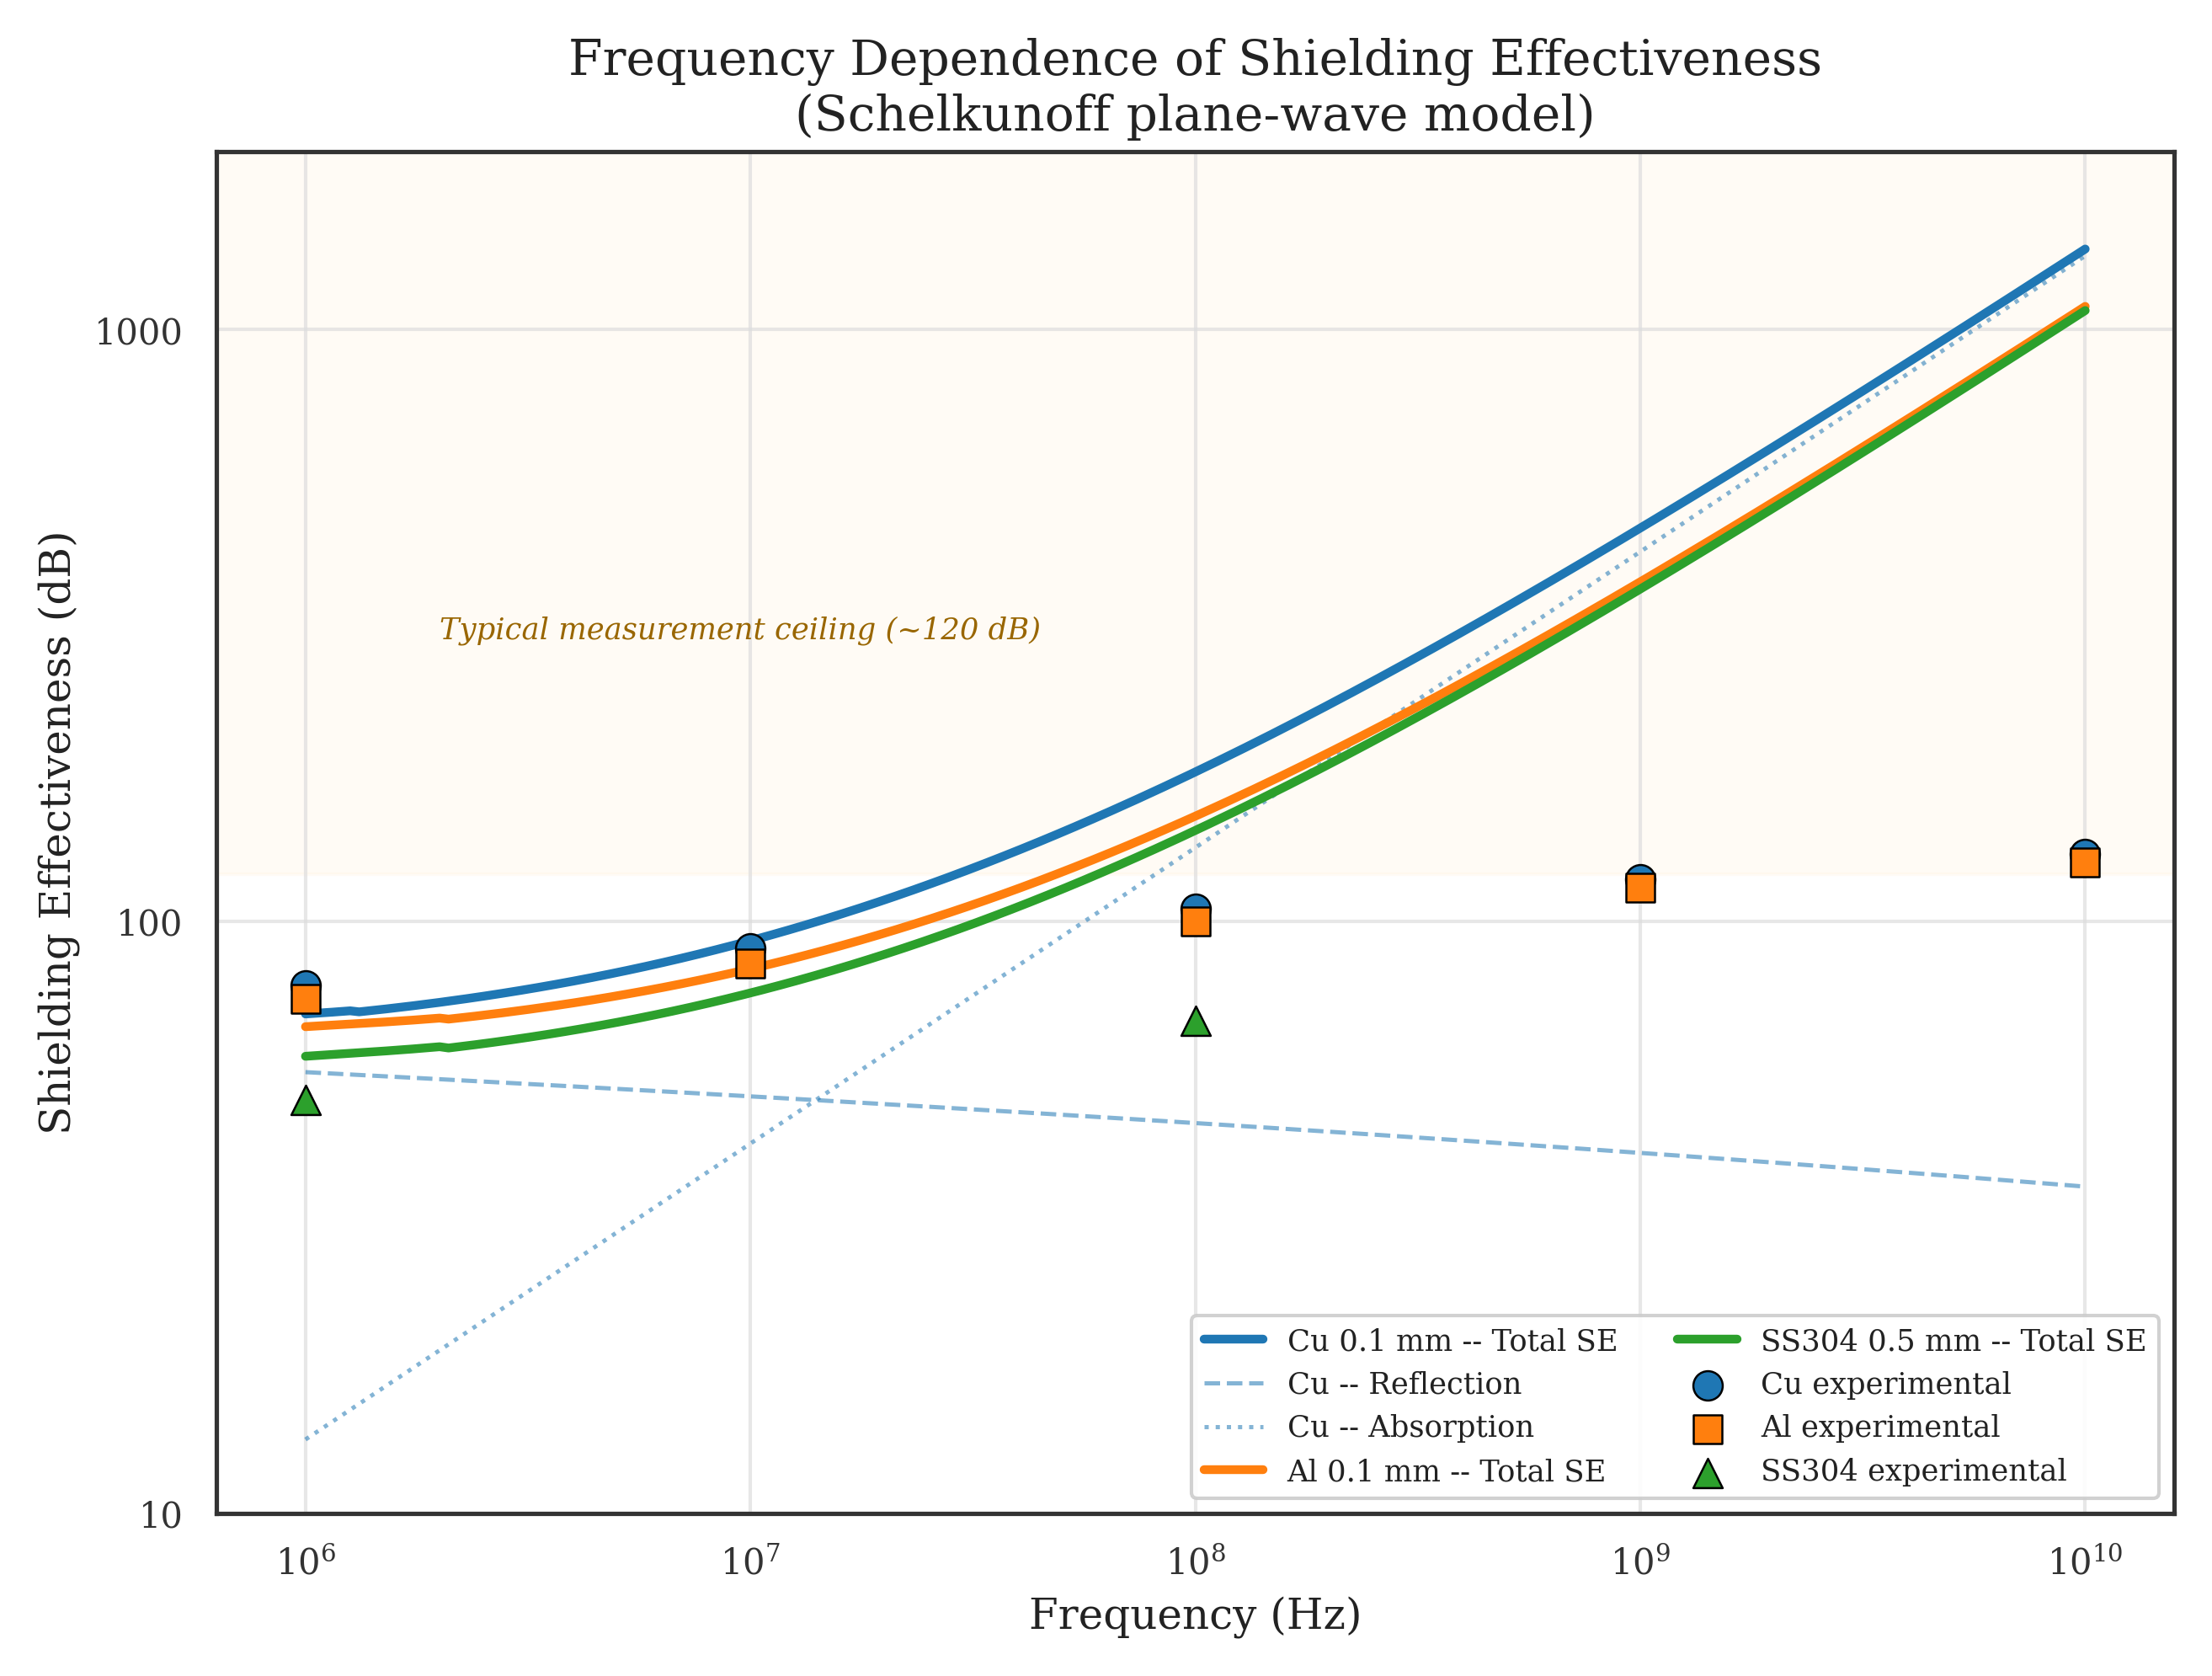
\includegraphics[width=0.85\textwidth]{figure4_frequency_sweep.png}
\caption{Frequency-dependent SE for copper (\SI{0.1}{mm}), aluminum (\SI{0.1}{mm}), and stainless steel 304 (\SI{0.5}{mm}). Solid lines: model predictions. Symbols: experimental benchmark data. Dashed lines: SE decomposition (reflection and absorption) for copper. Horizontal band at \SI{120}{dB}: typical measurement ceiling.}
\label{fig:sweep}
\end{figure}

\subsection{Multilayer weight reduction}

A Cu/PET/Cu sandwich was optimized via uniform thickness scaling for $SE \geq \SI{80}{dB}$ at \SI{10}{GHz}. The optimal configuration (\SI{12}{\micro m} Cu / \SI{500}{\micro m} PET / \SI{12}{\micro m} Cu) achieves $SE = \SI{82}{dB}$ at \SI{0.72}{kg/m^2}---approximately 10\% the weight of solid copper.

\subsection{Reliability-based composite design}

For a CNT/epoxy shield requiring $SE \geq \SI{40}{dB}$ at \SI{8.2}{GHz} with 95\% reliability: the deterministic threshold is 4.2~wt\% CNT, but the reliability-based threshold increases to 6.8~wt\% (a 62\% increase) to account for batch-to-batch variability near percolation.

%% ====================================================================
\section{Conclusions}
\label{sec:conclusions}
%% ====================================================================

An integrated analytical framework extending Schelkunoff theory with five coupled physics modules was presented and validated against 106 experimental benchmarks. The principal findings are:

\begin{enumerate}
\item For non-magnetic metals within the instrument-measurable range ($SE < \SI{90}{dB}$), the framework achieves MAE = \SI{6.6}{dB} and $R^2 = 0.68$. At higher SE values, theoretical predictions exceed measurement dynamic range, a fundamental limitation of comparing analytical plane-wave models against laboratory measurements.

\item The McLachlan GEM equation captures the sharp percolation transition in composite conductivity that linear mixing rules miss. However, composite SE prediction from bulk conductivity alone remains challenging (MAE = \SI{13}{dB}) for materials with anisotropic or lamellar microstructure, identifying internal structural effects as the key modelling frontier.

\item Sobol sensitivity analysis across material regimes reveals that the dominant uncertainty contributor is regime-dependent: permeability CV dominates for non-magnetic metals (counterintuitively), conductivity dominates near the percolation threshold, and grain size becomes competitive for nanocrystalline materials. This sensitivity crossover map is a new contribution with direct implications for manufacturing quality control.

\item Monte Carlo UQ with 95\% confidence intervals shows that reliability-based design requires 62\% higher filler loading than deterministic design for composites near percolation---a safety margin invisible to conventional single-point calculations.

\item Sub-second computation per evaluation enables integration with optimization and ML-driven materials discovery.
\end{enumerate}

Future work will integrate oblique-incidence corrections for enclosure-level SE, the Bloch--Gr\"uneisen conductivity model for cryogenic applications, anisotropic effective medium theory for aligned fiber composites, and Bayesian optimization for automated composite formulation discovery.

%% ====================================================================
\section*{CRediT authorship contribution statement}
%% ====================================================================

\textbf{Danush Arun:} Conceptualization, Methodology, Software, Validation, Formal analysis, Data curation, Writing -- original draft, Visualization.

%% ====================================================================
\section*{Declaration of competing interest}
%% ====================================================================

The authors declare that they have no known competing financial interests or personal relationships that could have appeared to influence the work reported in this paper.

%% ====================================================================
\section*{Acknowledgments}
%% ====================================================================

The author thanks Prof.\ [Supervisor Name] for guidance and critical review of the manuscript.

%% ====================================================================
\section*{Funding}
%% ====================================================================

This research did not receive any specific grant from funding agencies in the public, commercial, or not-for-profit sectors.

%% ====================================================================
\section*{Data availability}
%% ====================================================================

The benchmark dataset and simulation source code are available in the project repository. Supplementary Table~S1 contains the complete 106-entry benchmark dataset with literature citations for each measurement.

%% ====================================================================
%% REFERENCES
%% ====================================================================

\begin{thebibliography}{99}

\bibitem[Wanasinghe et al.(2020)]{Wanasinghe2020}
Wanasinghe, D., Aslani, F., Ma, G., Habibi, D., 2020.
Review of polymer composites with diverse nanofillers for electromagnetic interference shielding.
\textit{Nanomaterials} 10~(3), 541.
\url{https://doi.org/10.3390/nano10030541}

\bibitem[Hong et al.(2017)]{Hong2017}
Hong, W., Jiang, Z.H., Yu, C., et al., 2017.
Multibeam antenna technologies for 5G wireless communications.
\textit{IEEE J. Sel. Areas Commun.} 35~(6), 1291--1302.
\url{https://doi.org/10.1109/JSAC.2017.2687878}

\bibitem[Shahzad et al.(2016)]{Shahzad2016}
Shahzad, F., Alhabeb, M., Hatter, C.B., et al., 2016.
Electromagnetic interference shielding with 2D transition metal carbides (MXenes).
\textit{Science} 353~(6304), 1137--1140.
\url{https://doi.org/10.1126/science.aag2421}

\bibitem[Shen et al.(2014)]{Shen2014}
Shen, B., Zhai, W., Zheng, W., 2014.
Ultrathin flexible graphene film: An excellent thermal conducting material with efficient EMI shielding.
\textit{Adv. Funct. Mater.} 24~(28), 4542--4548.
\url{https://doi.org/10.1002/adfm.201400079}

\bibitem[Al-Saleh and Sundararaj(2009)]{AlSaleh2009}
Al-Saleh, M.H., Sundararaj, U., 2009.
Electromagnetic interference shielding mechanisms of CNT/polymer composites.
\textit{Carbon} 47~(7), 1738--1746.
\url{https://doi.org/10.1016/j.carbon.2009.02.030}

\bibitem[Ott(2009)]{Ott2009}
Ott, H.W., 2009.
\textit{Electromagnetic Compatibility Engineering}. Wiley.
\url{https://doi.org/10.1002/9780470508510}

\bibitem[Schulz et al.(1988)]{Schulz1988}
Schulz, R.B., Plantz, V.C., Brush, D.R., 1988.
Shielding theory and practice.
\textit{IEEE Trans. Electromagn. Compat.} 30~(3), 187--201.
\url{https://doi.org/10.1109/15.3297}

\bibitem[Schelkunoff(1934)]{Schelkunoff1934}
Schelkunoff, S.A., 1934.
The electromagnetic theory of coaxial transmission lines and cylindrical shields.
\textit{Bell Syst. Tech. J.} 13~(4), 532--579.
\url{https://doi.org/10.1002/j.1538-7305.1934.tb00679.x}

\bibitem[Kirkpatrick(1973)]{Kirkpatrick1973}
Kirkpatrick, S., 1973.
Percolation and conduction.
\textit{Rev. Mod. Phys.} 45~(4), 574--588.
\url{https://doi.org/10.1103/RevModPhys.45.574}

\bibitem[Stauffer and Aharony(1994)]{Stauffer1994}
Stauffer, D., Aharony, A., 1994.
\textit{Introduction to Percolation Theory}, second ed. Taylor \& Francis.
\url{https://doi.org/10.1201/9781315274386}

\bibitem[Arjmand et al.(2011)]{Arjmand2011}
Arjmand, M., Mahmoodi, M., Gelves, G.A., Park, S., Sundararaj, U., 2011.
Electrical and electromagnetic interference shielding properties of flow-induced oriented carbon nanotubes in polycarbonate.
\textit{Carbon} 49~(11), 3430--3440.
\url{https://doi.org/10.1016/j.carbon.2011.04.046}

\bibitem[Snoek(1948)]{Snoek1948}
Snoek, J.L., 1948.
Dispersion and absorption in magnetic ferrites at frequencies above one Mc/s.
\textit{Physica} 14~(4), 207--217.
\url{https://doi.org/10.1016/0031-8914(48)90038-X}

\bibitem[Celozzi et al.(2008)]{Celozzi2008}
Celozzi, S., Araneo, R., Lovat, G., 2008.
\textit{Electromagnetic Shielding}. Wiley.
\url{https://doi.org/10.1002/9780470268483}

\bibitem[Yeh(1988)]{Yeh1988}
Yeh, P., 1988.
\textit{Optical Waves in Layered Media}. Wiley.

\bibitem[Paul(2006)]{Paul2006}
Paul, C.R., 2006.
\textit{Introduction to Electromagnetic Compatibility}, second ed. Wiley.

\bibitem[Pozar(2011)]{Pozar2011}
Pozar, D.M., 2011.
\textit{Microwave Engineering}, fourth ed. Wiley.

\bibitem[Chung(2001)]{Chung2001}
Chung, D.D.L., 2001.
Electromagnetic interference shielding effectiveness of carbon materials.
\textit{Carbon} 39~(2), 279--285.
\url{https://doi.org/10.1016/S0008-6223(00)00184-6}

\bibitem[McLachlan et al.(1990)]{McLachlan1990}
McLachlan, D.S., Blaszkiewicz, M., Newnham, R.E., 1990.
Electrical resistivity of composites.
\textit{J. Am. Ceram. Soc.} 73~(8), 2187--2203.
\url{https://doi.org/10.1111/j.1151-2916.1990.tb07576.x}

\bibitem[Bauhofer and Kovacs(2009)]{Bauhofer2009}
Bauhofer, W., Kovacs, J.Z., 2009.
A review and analysis of electrical percolation in carbon nanotube polymer composites.
\textit{Compos. Sci. Technol.} 69~(10), 1486--1498.
\url{https://doi.org/10.1016/j.compscitech.2008.06.018}

\bibitem[Iqbal et al.(2020)]{Iqbal2020}
Iqbal, A., Shahzad, F., Hantanasirisakul, K., et al., 2020.
Anomalous absorption of electromagnetic waves by 2D transition metal carbonitride Ti$_3$CNT$_x$ (MXene).
\textit{Compos. Part B} 202, 108580.
\url{https://doi.org/10.1016/j.compositesb.2020.108580}

\bibitem[Sobol(2001)]{Sobol2001}
Sobol, I.M., 2001.
Global sensitivity indices for nonlinear mathematical models and their Monte Carlo estimates.
\textit{Math. Comput. Simul.} 55~(1--3), 271--280.

\bibitem[McKay et al.(1979)]{McKay1979}
McKay, M.D., Beckman, R.J., Conover, W.J., 1979.
A comparison of three methods for selecting values of input variables in the analysis of output from a computer code.
\textit{Technometrics} 21~(2), 239--245.

\bibitem[Cao et al.(2020)]{Cao2020}
Cao, M.S., Wang, X.X., Zhang, M., et al., 2020.
Electromagnetic response and energy conversion for functions and devices in low-dimensional materials.
\textit{Adv. Funct. Mater.} 30~(25), 1907698.
\url{https://doi.org/10.1002/adfm.201907698}

\bibitem[Han et al.(2020)]{Han2020}
Han, M., Shuck, C.E., Rakhmanov, R., et al., 2020.
Beyond Ti$_3$C$_2$T$_x$: MXenes for electromagnetic interference shielding.
\textit{ACS Nano} 14~(4), 11750--11759.
\url{https://doi.org/10.1021/acsnano.0c04504}

\bibitem[Balberg et al.(1984)]{Balberg1984}
Balberg, I., Anderson, C.H., Alexander, S., Wagner, N., 1984.
Excluded volume and its relation to the onset of percolation.
\textit{Phys. Rev. B} 30~(7), 3933.
\url{https://doi.org/10.1103/PhysRevB.30.3933}

\bibitem[Celzard et al.(1996)]{Celzard1996}
Celzard, A., McRae, E., Deleuze, C., et al., 1996.
Critical concentration in percolating systems containing a high-aspect-ratio filler.
\textit{Phys. Rev. B} 53~(10), 6209.
\url{https://doi.org/10.1103/PhysRevB.53.6209}

\bibitem[Li et al.(2015)]{Li2015}
Li, N., Huang, Y., Du, F., et al., 2015.
Electromagnetic interference (EMI) shielding of single-walled carbon nanotube epoxy composites.
\textit{Nanoscale} 7, 8219--8232.
\url{https://doi.org/10.1039/C5NR01083G}

\bibitem[Maxwell~Garnett(1904)]{MaxwellGarnett1904}
Maxwell~Garnett, J.C., 1904.
Colours in metal glasses and in metallic films.
\textit{Philos. Trans. R. Soc. Lond. Ser. A} 203, 385--420.
\url{https://doi.org/10.1098/rsta.1904.0024}

\bibitem[Bruggeman(1935)]{Bruggeman1935}
Bruggeman, D.A.G., 1935.
Berechnung verschiedener physikalischer Konstanten von heterogenen Substanzen.
\textit{Ann. Phys.} 416~(7), 636--664.
\url{https://doi.org/10.1002/andp.19354160705}

\bibitem[Hashin and Shtrikman(1962)]{Hashin1962}
Hashin, Z., Shtrikman, S., 1962.
A variational approach to the theory of the effective magnetic permeability of multiphase materials.
\textit{J. Appl. Phys.} 33~(10), 3125--3131.
\url{https://doi.org/10.1063/1.1728579}

\bibitem[Matula(1979)]{Matula1979}
Matula, R.A., 1979.
Electrical resistivity of copper, gold, palladium, and silver.
\textit{J. Phys. Chem. Ref. Data} 8~(4), 1147--1298.

\bibitem[Mayadas and Shatzkes(1970)]{Mayadas1970}
Mayadas, A.F., Shatzkes, M., 1970.
Electrical-resistivity model for polycrystalline films: The case of arbitrary reflection at external surfaces.
\textit{Phys. Rev. B} 1~(4), 1382--1389.
\url{https://doi.org/10.1103/PhysRevB.1.1382}

\bibitem[Saltelli(2002)]{Saltelli2002}
Saltelli, A., 2002.
Making best use of model evaluations to compute sensitivity indices.
\textit{Comput. Phys. Commun.} 145~(2), 280--297.

\bibitem[Hoang et al.(2015)]{Hoang2015}
Hoang, N.H., et al., 2015.
Effect of microstructure on electromagnetic shielding effectiveness of steel.
\textit{IEEE Trans. Electromagn. Compat.} 57~(6), 1566--1574.
\url{https://doi.org/10.1109/TEMC.2015.2460672}

\bibitem[Chung(2000)]{Chung2000}
Chung, D.D.L., 2000.
Materials for electromagnetic interference shielding.
\textit{J. Mater. Eng. Perform.} 9, 350--354.
\url{https://doi.org/10.1361/105994900770346042}

\bibitem[Luo and Chung(1999)]{Luo1999}
Luo, X., Chung, D.D.L., 1999.
Electromagnetic interference shielding using continuous carbon-fiber carbon-matrix and polymer-matrix composites.
\textit{Compos. Part B} 30~(3), 227--231.
\url{https://doi.org/10.1016/S1359-8368(98)00065-1}

\bibitem[Kim et al.(2008)]{Kim2008}
Kim, S.H., Jang, S.H., Byun, S.W., et al., 2008.
Electrical conductivity and electromagnetic interference shielding of Cu/PET multilayered composites.
\textit{Compos. Sci. Technol.} 68~(14), 2909--2916.
\url{https://doi.org/10.1016/j.compscitech.2007.10.024}

\bibitem[Thomassin et al.(2013)]{Thomassin2013}
Thomassin, J.M., J{\'e}r{\^o}me, C., Pardoen, T., Bailly, C., Huynen, I., Detrembleur, C., 2013.
Polymer/carbon based composites as electromagnetic interference (EMI) shielding materials.
\textit{Mater. Sci. Eng. R} 74~(7), 211--232.
\url{https://doi.org/10.1016/j.mser.2013.06.001}

\end{thebibliography}

\end{document}
